\chapter{Análisis y diseño}
\section{¿Qué es un agente?}
\subsection{Estructura de un agente}
\subsection{Comunicación entre agentes}

\newpage
\section{Planteamiento del problema}

\subsection{Cruce simple}
\begin{figure}[H]
    \centering
    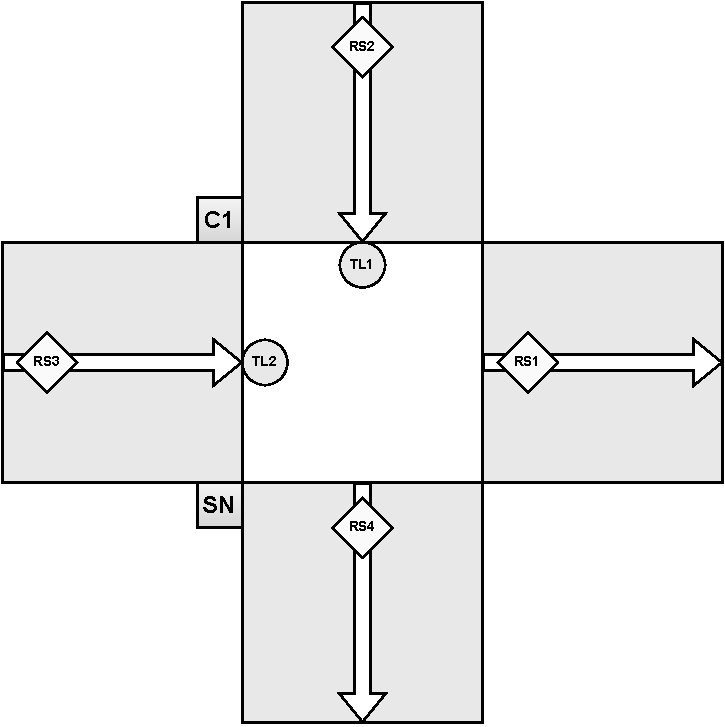
\includegraphics[width=1\linewidth]{text/image/DCruc-CS-Topologia.pdf}
    \caption{Topología del cruce simple}
    \label{fig:cruce_simple_topologia}
\end{figure}

\begin{figure}[H]
    \centering
    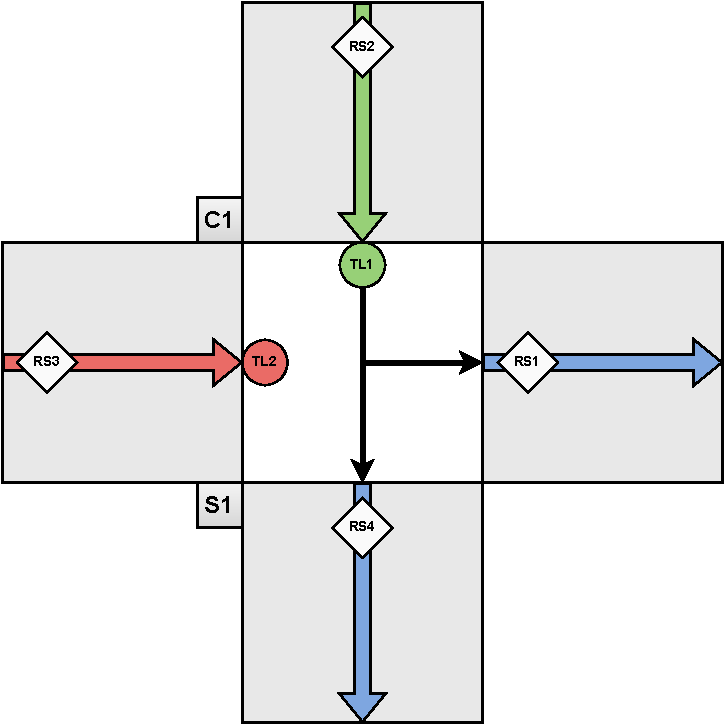
\includegraphics[width=1\linewidth]{text/image/DCruc-CS-Estado1.pdf}
    \caption{Cruce simple en estado 1}
    \label{fig:cruce_simple_estado_1}
\end{figure}

\begin{figure}[H]
    \centering
    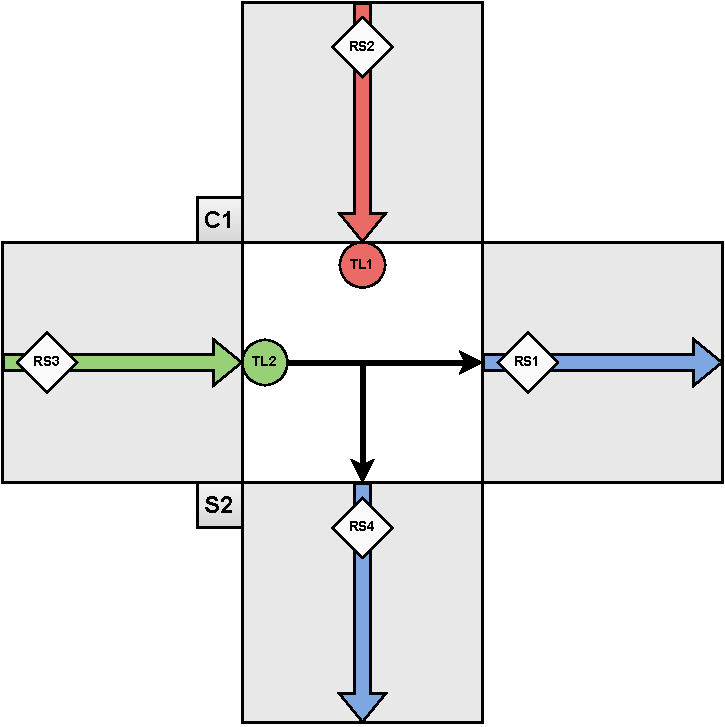
\includegraphics[width=1\linewidth]{text/image/DCruc-CS-Estado2.pdf}
    \caption{Cruce simple en estado 2}
    \label{fig:cruce_simple_estado_2}
\end{figure}

\newpage
\subsection{Cruce estándar}
\begin{figure}[H]
    \centering
    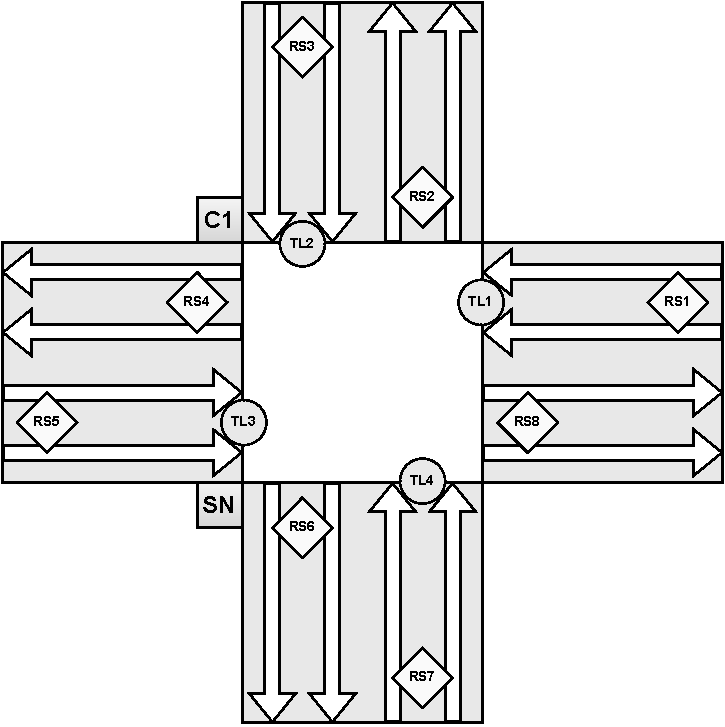
\includegraphics[width=1\linewidth]{text/image/DCruc-CE-Topologia.pdf}
    \caption{Topología del cruce estándar}
    \label{fig:cruce_estandar_topologia}
\end{figure}

\begin{figure}[H]
    \centering
    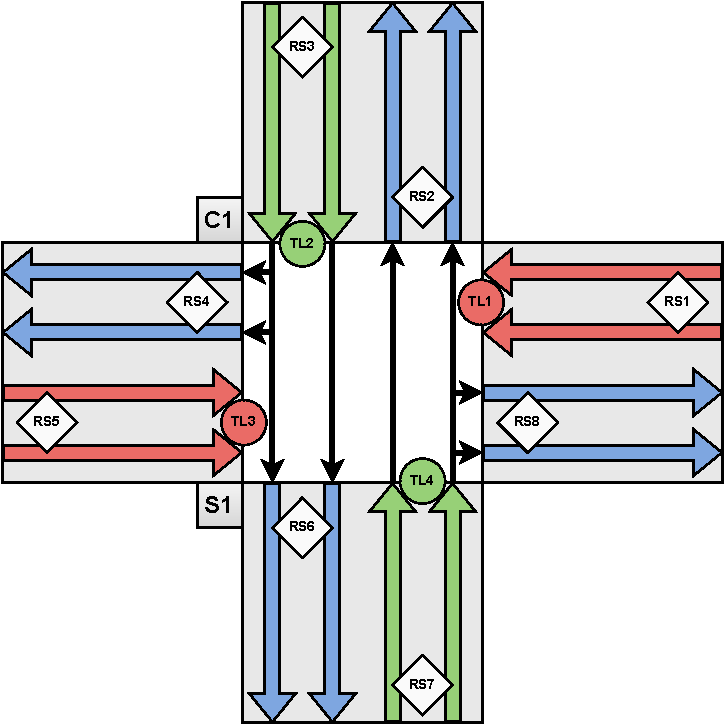
\includegraphics[width=1\linewidth]{text/image/DCruc-CE-Estado1.pdf}
    \caption{Cruce estándar en estado 1}
    \label{fig:cruce_estandar_estado_1}
\end{figure}

\begin{figure}[H]
    \centering
    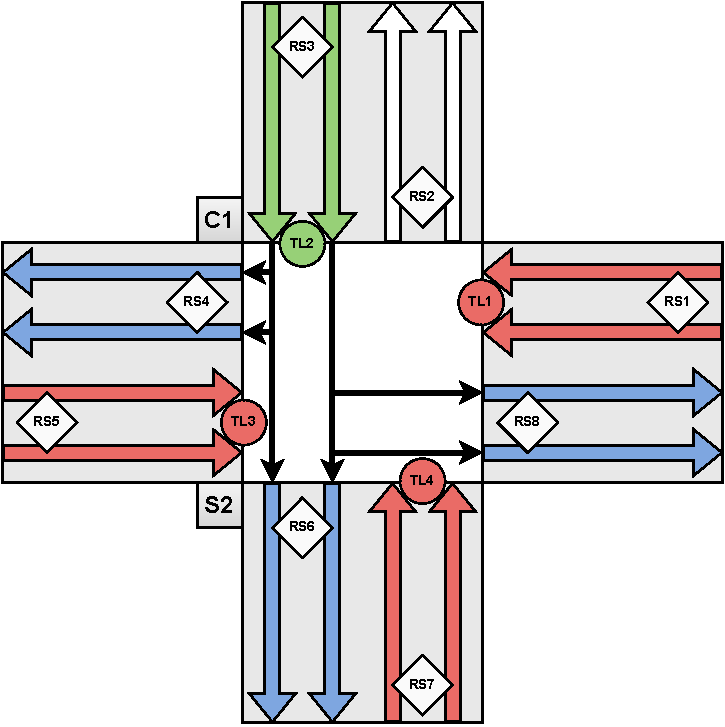
\includegraphics[width=1\linewidth]{text/image/DCruc-CE-Estado2.pdf}
    \caption{Cruce estándar en estado 2}
    \label{fig:cruce_estandar_estado_2}
\end{figure}

\begin{figure}[H]
    \centering
    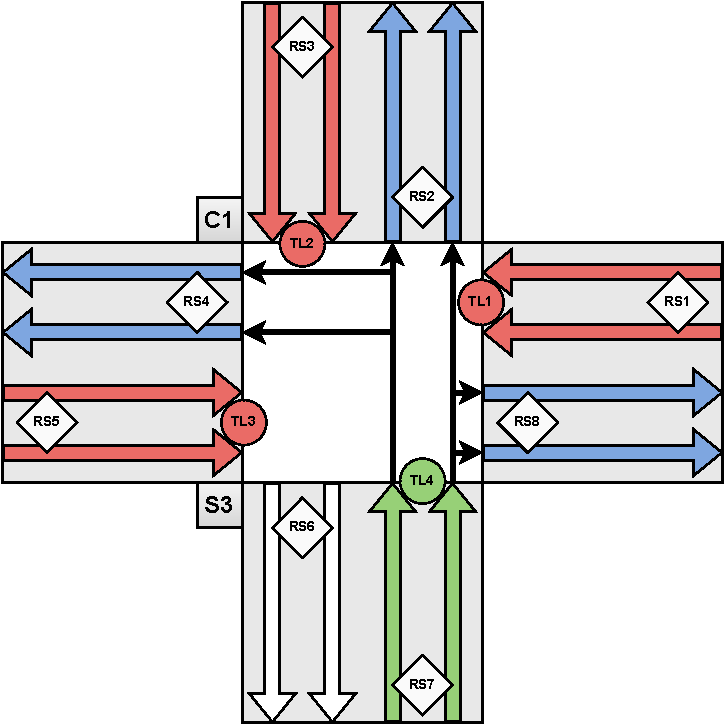
\includegraphics[width=1\linewidth]{text/image/DCruc-CE-Estado3.pdf}
    \caption{Cruce estándar en estado 3}
    \label{fig:cruce_estandar_estado_3}
\end{figure}

\begin{figure}[H]
    \centering
    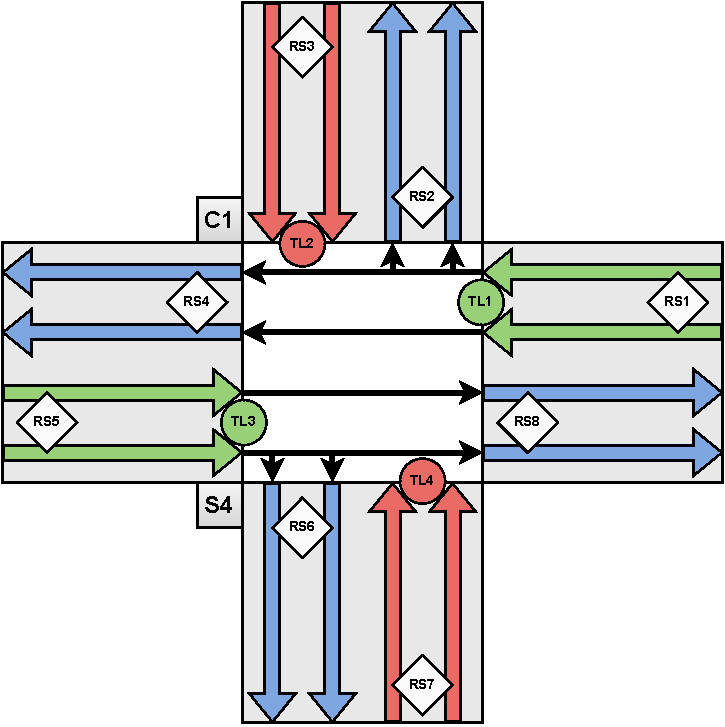
\includegraphics[width=1\linewidth]{text/image/DCruc-CE-Estado4.pdf}
    \caption{Cruce estándar en estado 4}
    \label{fig:cruce_estandar_estado_4}
\end{figure}

\begin{figure}[H]
    \centering
    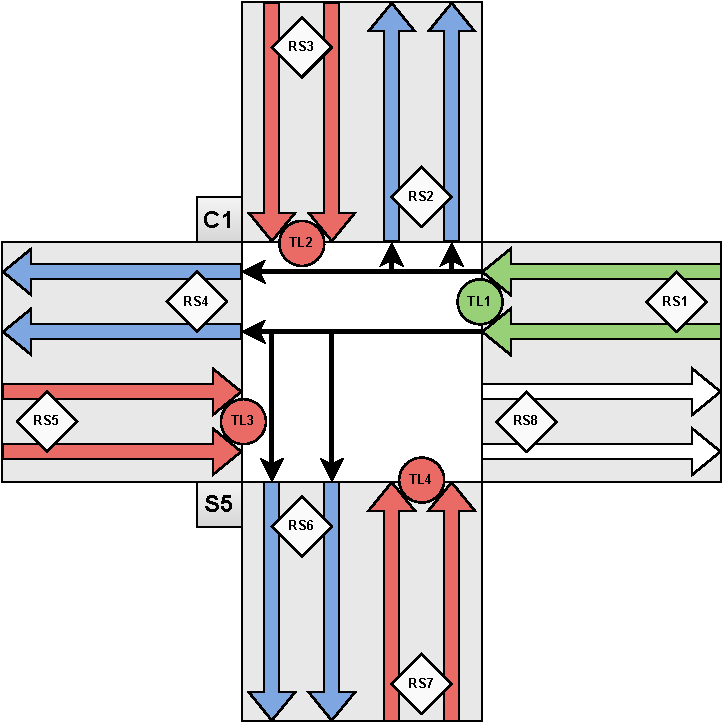
\includegraphics[width=1\linewidth]{text/image/DCruc-CE-Estado5.pdf}
    \caption{Cruce estándar en estado 5}
    \label{fig:cruce_estandar_estado_5}
\end{figure}

\begin{figure}[H]
    \centering
    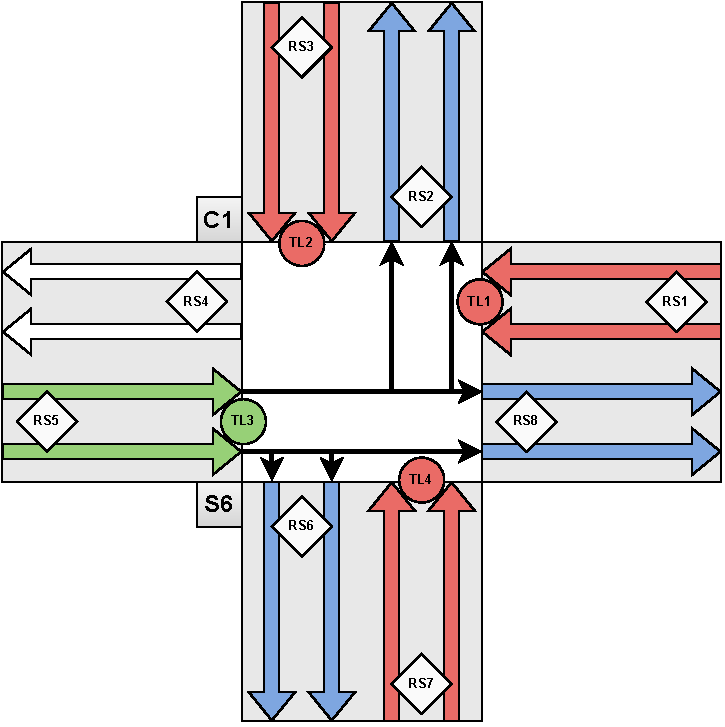
\includegraphics[width=1\linewidth]{text/image/DCruc-CE-Estado6.pdf}
    \caption{Cruce estándar en estado 6}
    \label{fig:cruce_estandar_estado_6}
\end{figure}

\newpage
\section{Sociedad de agentes}
El sistema MURAT es una construcción software basada en una arquitectura multiagente. Esto implica que existen uno o más tipos de agentes con roles definidos y propósitos específicos. Asimismo, existen uno o más agentes de cada tipo. Estos agentes, para el cumplimientos de sus objetivos, se encuentran organizados en una sociedad.

// TODO: Introducir sociedad de agentes

\begin{figure}[H]
    \centering
    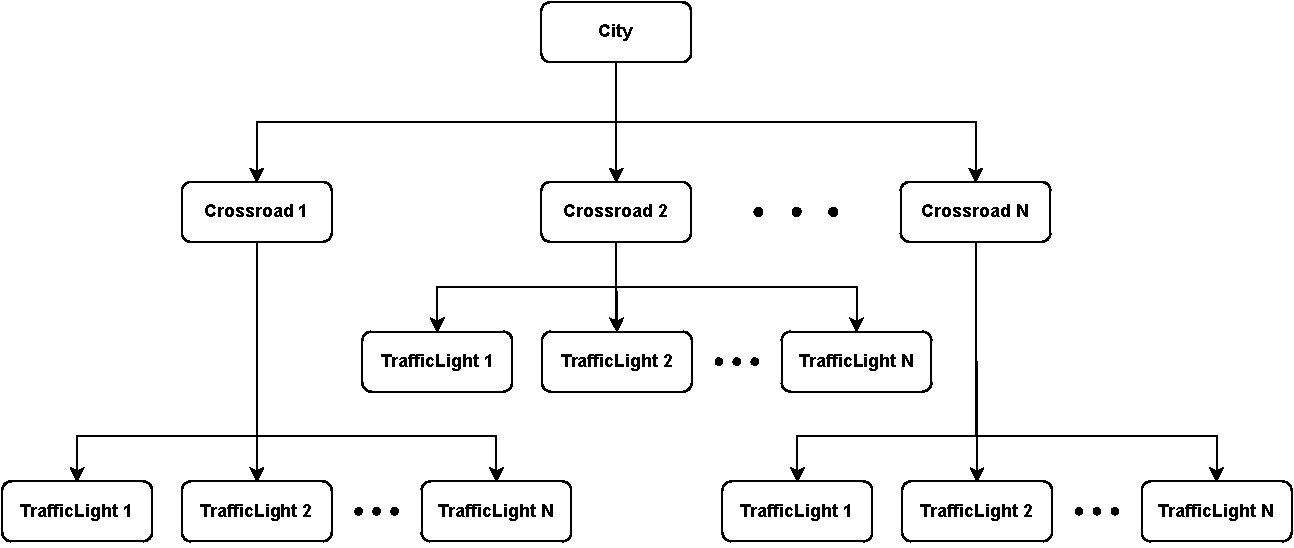
\includegraphics[width=1\linewidth]{text/image/DAgen-Sociedad_de_agentes.pdf}
    \caption{Sociedad de agentes del sistema MURAT}
    \label{fig:sociedad_de_agentes}
\end{figure}

\subsection{Agente Semáforo (TrafficLight)}
El agente \textit{Semáforo} es el agente más simple de la sociedad. Se encuentra en la posición menos privilegiada de la jerarquía. Opera a merced del único agente \textit{Cruce} que se encarga de él. Su capacidades son: cambiar su luz de rojo a verde o de verde a rojo; y poner la luz del color que haya ordenado el agente \textit{Cruce}. 

\subsubsection{Estados del agente}
\begin{enumerate}
    \item \textbf{Cargar datos} \footnotesize(LOAD\_DATA)\normalsize: Estado en el que se cargan los datos necesarios para el funcionamiento del agente.
    \begin{itemize}
        \item Se obtienen los datos del cruce al que pertenece.
        \item Se obtienen los datos del tramo de calle que regula.
    \end{itemize}
    Una vez se ha cargado la información el semáforo cambia al siguiente estado.
    \item \textbf{Escuchar al cruce} \footnotesize(LISTEN\_CROSSROAD)\normalsize: Estado en el que se escuchan mensajes para recibir mensajes provenientes del cruce. Mientras que el agente se encuentra en este estado permanece en una escucha continua de mensajes.
    \begin{itemize}
        \item Espera la inicialización por parte del agente \textit{Cruce}.
        \item TODO...
    \end{itemize}
    \item \textbf{Salir} \footnotesize(EXIT)\normalsize: Estado en el que el agente finaliza su ejecución. Un agente Semáforo nunca se podrá apagar si no es por orden del agente superior de la sociedad jerárquica a la que pertenece; siguiendo el flujo del software, a este estado solo se puede llegar tras la orden del agente Cruce.
\end{enumerate}

\subsubsection{Diagrama de actividad del agente}
\begin{figure}[H]
    \centering
    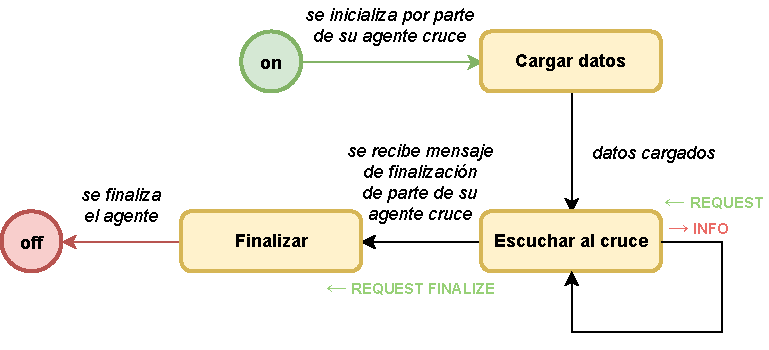
\includegraphics[width=1\linewidth]{text/image/DAgen-DA-TrafficLight.pdf}
    \caption{Diagrama de actividad del agente Semáforo}
    \label{fig:da_agente_semaforo}
\end{figure}

\subsection{Agente Cruce (Crossroad)}
\subsubsection{Estados del agente}


\subsection{Agente Ciudad (City)}

\renewcommand{\labelitemi}{$\bullet$}
\renewcommand{\labelitemii}{$\circ$}
\renewcommand{\labelitemiii}{$\Rightarrow$}

\newpage
\section{Modelo de datos de representación de la realidad}
En esta sección se expone el modelo de datos diseñado con el objetivo de realizar una representación precisa de la información del mundo real. Dicho modelo de datos es el nexo de unión entre las diferentes topologías de ciudades reales y sus correspondientes representaciones en el sistema MURAT. Este modelo de datos ha sido planteado de tal manera que permita representar desde una hasta varias ciudades, las cuales pueden poseer diferente complejidad.

\subsection{Representación en tablas}
La representación se realiza a través de un modelo basado en tablas, con un total de diez tablas:

\subsubsection{Tabla - Ciudad (\textit{city})}
En esta tabla se almacena la información básica, nombre y descripción, de las diferentes ciudades que están representadas y disponibles para ser simuladas en el sistema MURAT. \\\\
Atributos:
\begin{itemize}
    \item \textbf{Id de la ciudad} (\textit{city\_id}): identificador de la ciudad.
    \item \textbf{Nombre} (\textit{name}): nombre de la ciudad.
    \item \textbf{Descripción} (\textit{description}): descripción de la ciudad. Información extra de la ciudad.
\end{itemize}
\textbf{Clave primaria}: \{\textit{city\_id}\}. \\

\subsubsection{Tabla - Configuración de ciudad (\textit{city\_configuration})}
En esta tabla se almacena la información relativa a las diferentes configuraciones disponibles para cada ciudad. El sistema MURAT puede simular diferentes ciudades. Cada una de estas ciudades puede tener, a su vez, diferentes tipos de configuración. Por ejemplo, si para la misma ciudad se quieren realizar varias simulaciones que empiecen y/o terminen a horas diferentes se pueden crear y seleccionar diferentes tipos de configuración. O bien, si se desea que haya diferentes flujos de entrada de vehículos al sistema, también se pueden crear y elegir otras configuraciones.\\\\
Atributos:
\begin{itemize}
    \item \textbf{Id de la ciudad} (\textit{city\_id}): identificador de la ciudad.
    \item \textbf{Id de la configuración} (\textit{city\_configuration\_id}): identificador de la configuración.
    \item \textbf{Longitud de vehículo} (\textit{vehicle\_length}): longitud que mide un vehículo.
    \item \textbf{Ratio de entrada} (\textit{input\_ratio}): relación de entrada de tráfico al sistema. Cantidad de vehículos que se añaden a la simulación de tráfico por vía de tramo de calle y segundo.
    \item \textbf{Ratio interno de entrada} (\textit{input\_inner\_ratio}): relación de entrada de tráfico interna del sistema, es decir, desde unos cruces a otros cruces. Cantidad de vehículos que se mueven en un tramo de calle interno desde un cruce hasta otro cruce, es decir, número de vehículos que entran a los tramos de calle interiores (\textit{RoadStretchIn}) por vía y segundo.
    \item \textbf{Ratio interno de salida} (\textit{output\_inner\_ratio}): relación de salida de tráfico interna del sistema, es decir, o desde unos cruces hasta otros cruces o desde unos cruces hacia fuera del sistema. Cantidad de vehículos que salen, bien de tramos de calle entre cruces, bien de la simulación por vía y segundo.
    \item \textbf{Hora de inicio} (\textit{initial\_time}): hora de inicio de la simulación.
    \item \textbf{Hora de fin} (\textit{final\_time}): hora de fin de la simulación.
    \item \textbf{Tiempo de muestreo} (\textit{sample\_time}): tiempo de muestreo de la simulación. Cantidad de tiempo que pasa desde que se toma una muestra del estado de la simulación hasta que se toma la siguiente.
    \item \textbf{Modo} (\textit{mode}): modo en el que los vehículos se van añadiendo al sistema. En el sistema se contemplan tres valores:
    \begin{itemize}
        \item \textit{Lineal} (\textbf{LINEAR}): durante toda la simulación entra al sistema de tráfico la misma cantidad de vehículos.
        \item \textit{Pico único} (\textbf{SINGLE PEAK}): durante toda la simulación entra al sistema de tráfico la misma cantidad de vehículos a excepción de en un intervalo pico determinado, donde entra una cantidad mucho mayor. Esto, en la realidad se asemejaría, por ejemplo, al intervalo de 08:00 a 09:00, donde existe mayor afluencia de tráfico.
        \item \textit{Pico doble} (\textbf{DOUBLE PEAK}): durante toda la simulación entra al sistema de tráfico la misma cantidad de vehículos a excepción de en dos intervalos pico determinados, donde entran unas cantidades mucho mayores. Esto, en la realidad se asemejaría, por ejemplo, a los intervalos de 08:00 a 09:00 y de 19:00 a 20:00, donde existe mayor afluencia de tráfico.
    \end{itemize}
\end{itemize}
\textbf{Clave primaria}: \{\textit{city\_id}, \textit{city\_configuration\_id}\}. \\
\textbf{Clave foránea}: \{\textit{city\_id}\} de (\textit{city.city\_id}).

\subsubsection{Tabla - Estado inicial de cruces por configuración\\ (\textit{city\_configuration\_crossroad\_initial\_state})}
En esta tabla se almacena la información de los estados iniciales de cada cruce al inicio de la simulación de tráfico para cada configuración de cada ciudad. Ya se ha explicado que para cada ciudad pueden existir diferentes configuraciones. Cada una de estas configuraciones también define en qué estado está cada cruce al inicio de la simulación. Esta tabla se encarga de almacenar esa información. \\\\
Atributos:
\begin{itemize}
    \item \textbf{Id de la ciudad} (\textit{city\_id}): identificador de la ciudad.
    \item \textbf{Id de la configuración} (\textit{configuration\_id}): identificador de la configuración.
    \item \textbf{Id del cruce} (\textit{crossroad\_id}): identificador del cruce.
    \item \textbf{Id del estado inicial} (\textit{initial\_state\_id}): identificador del estado inicial.
\end{itemize}
\textbf{Clave primaria}: \{\{\textit{city\_id}, \textit{city\_configuration\_id}\}, \textit{crossroad\_id}\}. \\
\textbf{Claves foráneas}: Simples ya añadidas, \{\textit{city\_id}, \textit{city\_configuration\_id}\} \newline de (\textit{city\_configuration}) y \{\textit{crossroad\_id}\} de (\textit{crossroad.crossroad\_id}).

\subsubsection{Tabla - Cruce (\textit{crossroad})}
En esta tabla se almacena la información básica de los diferentes cruces de cada ciudad, los cuales están representados y disponibles para formar parte de una simulación del sistema MURAT. \\\\
Atributos:
\begin{itemize}
    \item \textbf{Id de la ciudad} (\textit{city\_id}): identificador de la ciudad.
    \item \textbf{Id del cruce} (\textit{crossroad\_id}): identificador del cruce.
    \item \textbf{Nombre} (\textit{name}): nombre del cruce.
    \item \textbf{Tiempo mínimo de estado} (\textit{minimum\_state\_time}): tiempo mínimo que debe durar cada uno de los estados de un cruce.
    \item \textbf{Tiempo de ciclo de estados} (\textit{cycle\_time}): tiempo que dura el paso entre todos los estados de un cruce, es decir, desde que un cruce inicia en un estado hasta que vuelve a ese mismo estado habiendo pasado por todos los demás.
\end{itemize}
\textbf{Clave primaria}: \{\textit{city\_id}, \textit{crossroad\_id}\}. \\
\textbf{Clave foránea}: \{\textit{city\_id}\} de (\textit{city.city\_id}).

\subsubsection{Tabla - Semáforo (\textit{traffic\_light})}
En esta tabla se almacena la información básica de los diferentes semáforos que hay en cada uno de los cruces de cada ciudad. Una de la simplificaciones del sistema MURAT es que los semáforos regulan únicamente la entrada de vehículos a un cruce, no la salida, por ello, cada semáforo tiene asociado un tramo de calle de entrada. \\\\
Atributos:
\begin{itemize}
    \item \textbf{Id de la ciudad} (\textit{city\_id}): identificador de la ciudad.
    \item \textbf{Id del cruce} (\textit{crossroad\_id}): identificador del cruce.
    \item \textbf{Id del semáforo} (\textit{traffic\_light\_id}): identificador del semáforo.
    \item \textbf{Nombre} (\textit{name}): nombre del semáforo.
    \item \textbf{Tramo de calle de entrada} (\textit{road\_stretch\_in}): tramo de calle de entrada al cruce regulado por el semáforo.
\end{itemize}
\textbf{Clave primaria}: \{\{\textit{city\_id}, \textit{crossroad\_id}\}, \textit{traffic\_light\_id}\}. \\
\textbf{Claves foráneas}: Simples ya añadidas, \{\textit{city\_id}, \textit{crossroad\_id}\} de (\textit{crossroad}) y \{\textit{road\_stretch\_in}\} de (\textit{road\_stretch.name}).

\subsubsection{Tabla - Estado (\textit{state})}
En esta tabla se almacena la información relativa a los diferentes estados en los que puede estar cada uno de los cruces de cada ciudad. En función del color en el que se encuentren los semáforos de un cruce, el cruce podría estar en un estado u otro. \\\\
Atributos:
\begin{itemize}
    \item \textbf{Id de la ciudad} (\textit{city\_id}): identificador de la ciudad.
    \item \textbf{Id del cruce} (\textit{crossroad\_id}): identificador del cruce.
    \item \textbf{Id del estado} (\textit{state\_id}): identificador del estado.
    \item \textbf{Nombre} (\textit{name}): nombre del estado.
    \item \textbf{Duración} (\textit{duration}): tiempo que dura el estado. El cruce permanece en un estado durante el tiempo que comprende la duración del mismo. Esta duración no puede ni ser inferior al tiempo mínimo de estado (\textit{minimum\_state\_time}) que define el cruce, ni exceder sumado a la duración del resto de estados el tiempo de ciclo de estados (\textit{cycle\_time}) que, también, define el cruce. 
\end{itemize}
\textbf{Clave primaria}: \{\{\textit{city\_id}, \textit{crossroad\_id}\}, {state\_id}\}. \\
\textbf{Claves foráneas}: Simples ya añadidas y \{\textit{city\_id}, \textit{crossroad\_id}\} de (\textit{crossroad}).

\subsubsection{Tabla - Luz de semáforos por estado (\textit{traffic\_light\_state})}
En esta tabla se almacena la información relativa al color de los semáforos para los diferentes estados posibles en los que puede estar cada uno de los cruces de cada ciudad. Como anteriormente se ha descrito, los estados de los cruces están definidos en función del color de los semáforos. Esta tabla es la que asocia cada estado con el color de cada uno de los semáforos. \\\\
Atributos:
\begin{itemize}
    \item \textbf{Id de la ciudad} (\textit{city\_id}): identificador de la ciudad.
    \item \textbf{Id del cruce} (\textit{crossroad\_id}): identificador del cruce.
    \item \textbf{Id del estado} (\textit{state\_id}): identificador del estado.
    \item \textbf{Id del semáforo} (\textit{traffic\_light\_id}): identificador del semáforo.
    \item \textbf{Luz del semáforo} (\textit{light}): color de la luz del semáforo.
\end{itemize}
\textbf{Clave primaria}: \{\{\textit{city\_id}, \textit{crossroad\_id}\}, \textit{state\_id}, \textit{traffic\_light\_id}\}. \\
\textbf{Claves foráneas}: Simples ya añadidas, \{\{\textit{city\_id}, \textit{crossroad\_id}\}, \textit{state\_id}\} de (\textit{state}) y \{\{\textit{city\_id}, \textit{crossroad\_id}\}, \textit{traffic\_light\_id}\} de (\textit{traffic\_light}).

\subsubsection{Tabla - Tramo de calle (\textit{road\_stretch})}
En esta tabla se almacena la información de los tramos de calle de cada ciudad. Cada calle real puede estar constituida por diferentes tramos de calle, que son cada uno de los carriles o conjunto de carriles que van desde un origen diferente hasta un destino igual o diferente y viceversa. \\\\
Atributos:
\begin{itemize}
    \item \textbf{Id de la ciudad} (\textit{city\_id}): identificador de la ciudad.
    \item \textbf{Id del cruce de origen} (\textit{crossroad\_origin\_id}): identificador del cruce de origen.
    \item \textbf{Id del cruce de destino} (\textit{crossroad\_destination\_id}): identificador del cruce de destino.
    \item \textbf{Dirección} (\textit{crossroad\_origin\_id}): dirección desde el cruce de origen hasta el cruce de destino expresada como dirección cardinal: N, NE, E, SE, S, SW, W o NW.
    \item \textbf{Nombre} (\textit{name}): nombre del tramo de calle.
    \item \textbf{Longitud} (\textit{length}): longitud del tramo de calle expresada en metros.
    \item \textbf{Carriles} (\textit{lanes}): número de carriles del tramo de calle.
    \item \textbf{Vehículos} (\textit{vehicles}): número de vehículos que hay en el tramo de calle.
\end{itemize}
Atributos calculados:
\begin{itemize}
    \item \textbf{Vehículos máximos} (\textit{max\_vehicles}): número máximo de vehículos que puede albergar un tramo de calle. Se calcula en base a tras atributos la longitud del tramo de calle, el número de carriles y la longitud por vehículo. Se multiplica la longitud del tramo por el número de carriles y se divide entre la longitud de vehículo.
    \item \textbf{Porcentaje de ocupación} (\textit{occupancy\_percentage}): porcentaje de ocupación del tramo de calle. Es la relación existente entre el número de vehículos que hay en el tramo de calle y el máximo de vehículos que caben en el mismo. Se calcula dividiendo el número de vehículos entre el número máximo de vehículos y multiplicando por cien.
    \item \textbf{Entrada de vehículos} (\textit{input}): cantidad de vehículos que pueden entrar al tramo de calle por segundo. Se calcula en función de su tipo, si es, o bien raíz (ratio de entrada), o bien cualquier otro, interno u hoja (ratio interno de entrada), multiplicando el ratio correspondiente por el número de carriles del tramo de calle.
    \item \textbf{Salida de vehículos} (\textit{output}): cantidad de vehículos que pueden salir de tramo de calle por segundo. Se calcula multiplicando el ratio interno de salida por el número de carriles del tramo de calle.
    \item \textbf{Tipo} (\textit{type}): tipo de tramo de calles. Se identifican los tres siguientes tipos de tramos de calle en función de los valores de los atributos cruce de origen y cruce de destino.
    \begin{itemize}
        \item Si \textbf{no} existe el \textbf{cruce de origen} y existe el \textbf{cruce de destino} se trata de un tramo de calle raíz (\textbf{ROOT}), es decir, un tramo de calle por el que entran vehículos al sistema.
        \item Si existe el \textbf{cruce de origen} y \textbf{no} existe el \textbf{cruce destino} se trata de un tramo de calle hoja (\textbf{LEAF}), es decir, un tramo de calle por el que salen vehículos del sistema.
        \item Si existe el \textbf{cruce de origen} y existe el \textbf{cruce destino} se trata de un tramo de calle interno (\textbf{INNER}), es decir, un tramo de calle por el los vehículos pasan de un cruce a otro.
    \end{itemize}
\end{itemize}
\textbf{Clave primaria}: \{\textit{city\_id}, \{\textit{origin\_crossroad\_id}, \textit{destionation\_crossroad\_id}\}. \\
\textbf{Claves foráneas}: Simples ya añadidas, \{\textit{origin\_crossroad\_id}\} de (\textit{crossroad\_id}) y \{\textit{destination\_crossroad\_id}\} de (\textit{crossroad\_id}).

\subsubsection{Tabla - Tramo de cruce (\textit{crossroad\_stretch})}
En esta tabla se almacena la información de los tramos de cruce de cada uno de los cruces de cada ciudad. Los vehículos, a través del cruce, tienen que ir desde un tramo de calle hasta otro tramo de calle. Esta ruta es a lo que se le llama tramo de cruce. Esta tabla se asemeja a un router que para cada tramo de calle de origen enruta los vehículos a uno o varios tramos de calle de destino. \\\\
Atributos:
\begin{itemize}
    \item \textbf{Id de la ciudad} (\textit{city\_id}): identificador de la ciudad.
    \item \textbf{Id del cruce} (\textit{crossroad\_id}): identificador del cruce.
    \item \textbf{Nombre del tramo de calle de origen} (\textit{road\_strech\_origin\_name}): tramo de calle de origen del vehículo.
    \item \textbf{Nombre del tramo de calle de destino} (\textit{road\_strech\_destination\_name}): tramo de calle de destino del vehículo.
    \item \textbf{Nombre} (\textit{name}): nombre del tramo de cruce. Está formado por la concatenación del nombre del tramo de calle de origen, el separador <<->> y el nombre del tramo de calle de destino.
    \item \textbf{Porcentaje de coches que van de origen a destino}\\ (\textit{cars\_percentage\_from\_origin\_to\_destination}): porcentaje de vehículos interesados en ir desde el tramo de calle de origen hasta el tramo de calle de destino. Desde un tramo de calle de origen se puede ir hacia uno o varios diferentes tramos de calle destino. Cada uno de estos tramos de cruce tendrá un porcentaje de vehículos interesados. La suma de los porcentajes de vehículos cuyos tramos de cruce tienen el mismo origen deben sumar 100\%. Es como decir qué porcentaje de vehículos están interesados en ir desde un origen hasta cada uno de sus destinos. Si desde un origen solo se puede ir hasta un destino, el porcentaje de vehículos interesados es del 100\%. Si desde un origen se pueden ir hacia dos destinos: el primero de ellos una calle principal, muy grande; y el segundo de ellos una calle secundaria, más pequeña; sería una situación racional que el 85\% estuvieran interesados en ir hacia el primer destino y el 15\% restante hacia el segundo destino. 
\end{itemize}
\textbf{Clave primaria}: \{\{\textit{city\_id}, \textit{crossroad\_id}\}, \textit{origin\_road\_stretch\_name}, \textit{destination\_road\_stretch\_name}\}. \\
\textbf{Claves foráneas}: Simples ya añadidas, \{\textit{city\_id}, \textit{crossroad\_id}\} de (\textit{crossroad}), \{\textit{origin\_road\_stretch\_name}\} de (\textit{road\_stretch.road\_stretch\_name}) \newline y \{\textit{destination\_road\_stretch\_name}\} de (\textit{road\_stretch.road\_stretch\_name}).

\subsubsection{Tabla - Rutas de tramos de cruce (\textit{crossroad\_stretch\_routes})}
En esta tabla se almacena la información de los tramos de cruce que habilita cada uno de los semáforos en verde para cada estado de cada uno de los cruces de cada ciudad. Que un semáforo esté en verde significa que los vehículos puedan pasar desde un tramo de calle origen hasta uno o varios tramos de calle destino. Esta tabla es la encargada de almacenar esa información. \\\\
Atributos:
\begin{itemize}
    \item \textbf{Id de la ciudad} (\textit{city\_id}): identificador de la ciudad.
    \item \textbf{Id del cruce} (\textit{crossroad\_id}): identificador del cruce.
    \item \textbf{Id del estado} (\textit{state\_id}): identificador del estado.
    \item \textbf{Id del semáforo} (\textit{traffic\_light\_id}): identificador del semáforo.
    \item \textbf{Nombre del tramo de cruce} (\textit{crossroad\_stretch\_name}): nombre del tramo de cruce. Está formado por la concatenación del nombre del tramo de calle de origen, el separador <<->> y el nombre del tramo de calle de destino.
\end{itemize}
\textbf{Clave primaria}: \{\{\textit{city\_id}, \textit{crossroad\_id}\}, \textit{state\_id}, \textit{traffic\_light\_id}\}. \\
\textbf{Claves foráneas}: Simples ya añadidas, \{\{\textit{city\_id}, \textit{crossroad\_id}\}, \textit{state\_id}\} de (\textit{state}), \{\{\textit{city\_id}, \textit{crossroad\_id}\}, \textit{traffic\_light\_id}\} de (\textit{traffic\_light}) y \newline \{\textit{crossroad\_stretch\_name}\} de (\textit{crossroad\_stretch.name}).

\subsection{Representación en JSON}
La representación se realiza a través de un objeto de tipo JSON basado en las tablas anteriormente descritas.

//TODO: explicar
\lstinputlisting[language=json, linerange={1-10}]{text/data/CITY1.json}

\subsection{Carga de datos en la inicialización}
El sistema MURAT se sirve en su arranque de información que representa a una ciudad junto a sus calles, cruces y semáforos, además de la información de su configuración, variables relativas a la simulación de tráfico en la ciudad. Los datos cargados en el sistema para realizar una simulación de tráfico se indexan por el identificador de ciudad e identificador de configuración a través de la selección de uno de los archivos \textit{.json} existentes y una de sus configuraciones.